\documentclass[border=6pt]{standalone}
\usepackage{tikz}
\usepackage[edges]{forest}
\usetikzlibrary{arrows.meta,positioning,calc,decorations.pathreplacing,shapes.geometric}
\begin{document}
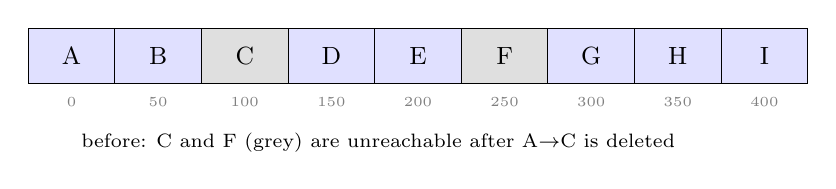
\begin{tikzpicture}[>=Stealth,font=\small]
\node[draw,minimum width=1.10cm,minimum height=0.7cm,fill=blue!12] (a) at (0.00,0.00) {A};
\node[draw,minimum width=1.10cm,minimum height=0.7cm,fill=blue!12] (b) at (1.10,0.00) {B};
\node[draw,minimum width=1.10cm,minimum height=0.7cm,fill=gray!25] (c) at (2.20,0.00) {C};
\node[draw,minimum width=1.10cm,minimum height=0.7cm,fill=blue!12] (d) at (3.30,0.00) {D};
\node[draw,minimum width=1.10cm,minimum height=0.7cm,fill=blue!12] (e) at (4.40,0.00) {E};
\node[draw,minimum width=1.10cm,minimum height=0.7cm,fill=gray!25] (f) at (5.50,0.00) {F};
\node[draw,minimum width=1.10cm,minimum height=0.7cm,fill=blue!12] (g) at (6.60,0.00) {G};
\node[draw,minimum width=1.10cm,minimum height=0.7cm,fill=blue!12] (h) at (7.70,0.00) {H};
\node[draw,minimum width=1.10cm,minimum height=0.7cm,fill=blue!12] (i) at (8.80,0.00) {I};
\node[font=\tiny,gray,below=0.05cm of a] {0};
\node[font=\tiny,gray,below=0.05cm of b] {50};
\node[font=\tiny,gray,below=0.05cm of c] {100};
\node[font=\tiny,gray,below=0.05cm of d] {150};
\node[font=\tiny,gray,below=0.05cm of e] {200};
\node[font=\tiny,gray,below=0.05cm of f] {250};
\node[font=\tiny,gray,below=0.05cm of g] {300};
\node[font=\tiny,gray,below=0.05cm of h] {350};
\node[font=\tiny,gray,below=0.05cm of i] {400};
\node[font=\scriptsize,anchor=west] at (0,-1.1) {before: C and F (grey) are unreachable after A$\to$C is deleted};
\end{tikzpicture}
\end{document}
